% Full draft for a conference / journal submission — generic template (plain article class). To move to a venue class
% (IEEEtran, acmart, llncs, ...), keep the body and replace the preamble and the front matter.
% Build:  latexmk -pdf main.tex
% Figures: figures/paper_figures.ipynb (style: figures/paper_style.py; dataset_construction.py runs on the server)
% Notes for the authors would be in \todo{...} (red). The previous draft is in _da_cancellare/.
\documentclass[11pt,a4paper]{article}
\usepackage[margin=2.5cm]{geometry}
\usepackage[T1]{fontenc}
\usepackage[utf8]{inputenc}
\usepackage{lmodern}
\usepackage{amsmath,amssymb}
\usepackage{graphicx}
\usepackage{booktabs}
\usepackage{xcolor}
\usepackage{tikz}
\usetikzlibrary{arrows.meta,positioning,shapes.misc}
\usepackage[numbers,sort&compress]{natbib}
\usepackage{xr-hyper}
\usepackage[colorlinks=true,linkcolor=blue!50!black,citecolor=blue!50!black,urlcolor=blue!50!black]{hyperref}
\def\UrlBreaks{\do\/\do-\do\_\do.}
\usepackage{authblk}
\usepackage{orcidlink}
\renewcommand\Affilfont{\small}

\externaldocument[S-]{supplementary}
\newcommand{\todo}[1]{\textcolor{red}{[\textbf{TODO:} #1]}}
\newcommand{\anon}{\operatorname{anon}}

\title{Traces of Reliability: Predicting the Rating of Unseen News Publishers from the Anonymized Text
of Their Articles}
\author[1]{John Bianchi\,\orcidlink{0009-0006-2582-1480}\thanks{Corresponding author: John Bianchi
(\texttt{john.bianchi@imtlucca.it}).}}
\author[2]{Manuel Pratelli\,\orcidlink{0000-0002-9978-791X}}
\author[1]{Fabio Pinelli\,\orcidlink{0000-0003-1058-6917}}
\author[2,1]{Marinella Petrocchi\,\orcidlink{0000-0003-0591-877X}}
\affil[1]{IMT School for Advanced Studies Lucca, 55100 Lucca, Italy\\
\texttt{\{john.bianchi, fabio.pinelli\}@imtlucca.it}}
\affil[2]{Institute of Informatics and Telematics, National Research Council (IIT-CNR), 56124 Pisa, Italy\\
\texttt{\{manuel.pratelli, marinella.petrocchi\}@iit.cnr.it}}
\date{}

\begin{document}
\maketitle

\begin{abstract}
Professional raters such as NewsGuard judge a news outlet by how it works: whether it publishes false content, corrects
its errors, separates news from opinion and discloses who owns it. These practices are checked outside the articles,
but they may leave a trace in everything an outlet writes. We ask whether this trace is enough to predict the rating of
an outlet that a model has never seen, after removing from its articles everything that names it. We collect 25,524
articles from 226 English-language political outlets rated by NewsGuard, remove the articles copied across outlets, keep
one outlet per owner, and replace links, e-mail addresses and the names of outlets and journalists with placeholders. A
model scores each article, and the score of an outlet is the mean over its articles. With a ridge regression on the
hidden states of the frozen Mistral-Small-24B, the predicted NewsGuard score (0--100) of an unseen outlet is off by 15.8
points on average, against 17.8 for TF-IDF and 22.1 for a constant prediction. Few articles are needed: with five
articles per outlet, Mistral-Small-24B is already more accurate than TF-IDF reading all the articles of each outlet. Only
large models capture the trace, since small encoders, frozen or fine-tuned, are no better than TF-IDF, and asking the
model for the score directly works poorly. Masking the names changes the error by less than half a point, while letting
the same outlet or its sister sites into training lowers it by 6--12 points, so weaker evaluation protocols overstate
the results. Finally, the models predict about 9 points more for a left-leaning outlet than for a right-leaning outlet
with the same NewsGuard score. We release the code, the models, the predictions and a local tool.
\end{abstract}

\noindent\textbf{Keywords:} news source reliability; publisher reliability inference; media profiling; anonymization;
large language models; text regression; NewsGuard.

% =====================================================================================================================
\section{Introduction}\label{sec:intro}

In contemporary digital media ecosystems, assessing the reliability of news publishers has become an important means
of limiting the spread of misleading or low-quality information~\cite{Bowman2003,Jemielniak2020}. Organizations such as
NewsGuard, the Global Disinformation Index and Media Bias/Fact Check rate news outlets on journalistic standards such as
transparency, editorial accountability, factual accuracy and corrections, and their ratings largely
agree~\cite{lin2023high,DBLP:conf/icwsm/PratelliP22}. Each rating is made by trained journalists, outlet by outlet, so
many outlets, especially new and small ones, remain unrated for a long time.

Automatic methods could help. Many predict credibility from articles~\cite{pandolfi2020automatic,Przybyla2021plugin,
10.1145/3770077,DBLP:journals/dbsk/AdjiLS26} or profile media sources from their articles and other
signals~\cite{baly2018predicting,baly2020written,nakov2024survey}. When the labels come from ratings of publishers,
however, two problems can make the results look better than they are. First, if the same publisher is in the training
and in the test data, a model can learn to recognize the publisher instead of learning what makes it
reliable~\cite{zhou2021hidden,azizov-etal-2024-safari,verhoeven2025yesterday}. Second, even with different publishers
in training and test, the text often reveals its source: the outlet's name, the names of its journalists, the links to
its own pages and, as we show in Section~\ref{sec:groups}, whole articles copied across sites of the same owner. In both
cases a model can recognize an outlet without judging its writing. In previous work we classified articles into the
reliability levels of their publishers~\cite{Bianchi2024SAC}. Here we remove both problems.

Our question is simple: can the NewsGuard score of an outlet that the model has never seen be predicted from its
articles once every name has been removed? The answer is not obvious, because NewsGuard checks its criteria outside the
articles, for instance by verifying claims against other sources or by reading the \emph{about} page of an outlet for
its ownership and financing. Still, the way an outlet works may leave traces in how it writes: how it sources and hedges
claims, whether it separates news from opinion, which topics it covers and in what tone. We look for these traces, and
not for the identity of the outlet.

We treat the problem as a regression at the level of the publisher. A model predicts a score for each article, and the
score of a publisher is the mean of the predictions for its articles, so the judgment on an outlet always rests on
several articles. The evaluation follows four rules: the test outlets never appear in training, outlets of the same
owner are never split between training and test, articles copied across outlets are removed, and every article is
anonymized before any model reads it. Our contributions are:
\begin{enumerate}
  \item A dataset of 25,524 articles from 226 English-language political outlets with NewsGuard scores, built with a few
        explicit filters (language, length, date, duplicates, one outlet per owner). We show that copied articles almost
        always link outlets of the same owner, and that a single network of 164 sites would otherwise fill the least
        reliable level (Section~\ref{sec:data}).
  \item An anonymization that masks the outlet's own name and, with a zero-shot named-entity recognizer, every outlet and
        journalist in the text (Section~\ref{sec:anon}).
  \item A comparison of TF-IDF, frozen language models from 0.6 to 24 billion parameters, a fine-tuned encoder and a
        zero-shot model. The large frozen models are the most accurate, with an error up to 2 points lower than TF-IDF
        for any number of articles per outlet (Sections~\ref{sec:setup}--\ref{sec:k}).
  \item A measure of how much each rule of the protocol matters: splitting articles instead of outlets, or training on
        outlets of the same owner, lowers the error by 6--12 points, while masking the names changes it by less than
        half a point (Section~\ref{sec:ladder}).
  \item An analysis of the errors by reliability level and political orientation, and the release of the code, the
        models, the predictions and a local tool (Sections~\ref{sec:errors}--\ref{sec:tool}).
\end{enumerate}

% =====================================================================================================================
\section{Related Work}\label{sec:related}

\paragraph{Publisher reliability.} Credibility is often assessed article by article~\cite{pandolfi2020automatic,
10.1145/3770077}, but the reputation of the source strongly shapes how information is
perceived~\cite{doi:10.1080/07421222.2019.1628921}. The ratings of NewsGuard, the Global Disinformation Index and Media
Bias/Fact Check (MBFC) largely agree and are widely used as ground truth~\cite{lin2023high,DBLP:conf/icwsm/PratelliP22}.
The reliability of a publisher has been predicted from writing style~\cite{przybyla2020capturing,potthast2018stylometric},
from user interactions, social networks, web graphs and
metadata~\cite{bazmi2023multi,DBLP:conf/ecir/PratelliSP25,DBLP:conf/icwsm/WilliamsCC25,DBLP:journals/jdiq/LongoZCZC25},
and from articles combined with Wikipedia, social media and audience
data~\cite{baly2018predicting,baly2020written,nakov2024survey}. Large language models have also been asked to rate named
sources~\cite{yang2023large} or to produce weak credibility labels~\cite{Leite2025}. Given the name of a source, however,
a model may simply recall what it knows about it, which is why we mask the names.

\paragraph{Evaluation on unseen sources.} Zhou et al.~\cite{zhou2021hidden} showed that models trained on labels
inherited from the sources learn the sources themselves, and that random splits of the articles overestimate
performance. Later work found that performance drops under shifts of domain, time and
publisher~\cite{azizov-etal-2024-safari,burdisso-etal-2024-reliability,verhoeven2025yesterday}. Table~\ref{tab:related}
compares the studies closest to ours, which predict reliability mainly from text with labels given to the sources. All those that compare seen with unseen sources report a drop: from 0.91 to 0.65 F1 in Rashkin et al.~\cite{rashkin2017truth},
from 0.94 to 0.86 AUC in Horne et al.~\cite{horne2019robust}, from 0.998 to 0.796 accuracy in
Przyby{\l}a~\cite{przybyla2020capturing} and from 0.97 to 0.72 AUC in Bozarth and Budak~\cite{bozarth2020toward}. None
of them keeps the outlets of the same owner apart, although outlets often share
content~\cite{horne2019spirals,gruppi2021tell}, only Bozarth and Budak remove the names of the outlets, and all predict
classes. Continuous reliability has been estimated from the links between news sites~\cite{burdisso-etal-2024-reliability}
and from the web graph, the text and time~\cite{kondrup2026credibench}, and Eldifrawi et al.~\cite{eldifrawi2026temporal} classify the credibility of domains, without their names, from the
judgments of a language model on their articles, with evidence from web search, aggregated by a decision tree. We predict the full 0--100
score from the anonymized text alone, under all the protections above. Datasets with source-level labels include
NELA-GT~\cite{gruppi2021nela}, a Czech dataset~\cite{bohavcek2022fine} and the BAT
corpus~\cite{DBLP:journals/dbsk/AdjiLS26,batDataset}, and splits by publisher were already used in the hyperpartisan
task of SemEval-2019~\cite{kiesel2019semeval}.

\begin{table}[t]
\centering\small
\caption{Comparison with the closest studies. Each row is a study and each column a property of its setting: what the model reads (\emph{other}: Wikipedia, Twitter, URL and traffic for Baly et al., backlinks and page design for
Eldifrawi et al.; \emph{links}: a separate model on the links between domains, which predicts per domain), where the
labels come from, whether the test sources are absent from training (\emph{in part}: in one experiment), whether outlets
of the same owner are kept on the same side of the split, which names are removed from the text (\emph{all}: outlets,
journalists, links and e-mail addresses), and what is predicted. --: not done or not reported.}\label{tab:related}
\footnotesize\setlength{\tabcolsep}{3.5pt}
\resizebox{\linewidth}{!}{%
\begin{tabular}{lllllll}
\toprule
study & input & labels & unseen & owners & names & target \\
 & & & sources & apart & masked & \\
\midrule
Rashkin et al.~\cite{rashkin2017truth} & text & source type & yes & -- & -- & 4 classes per article \\
Baly et al.~\cite{baly2018predicting} & text + other & MBFC & yes & -- & -- & 3 classes per source \\
Fairbanks et al.~\cite{fairbanks2018credibility} & text; links & MBFC & -- & -- & -- & 2 classes per article \\
Horne et al.~\cite{horne2019robust} & text + Wikipedia & NewsGuard, OpenSources & in part & -- & -- & 2 classes per article \\
Przyby{\l}a~\cite{przybyla2020capturing} & text & PolitiFact, Pew & in part & -- & -- & 2 classes per article \\
Bozarth \& Budak~\cite{bozarth2020toward} & text or social & MBFC & in part & -- & outlets & 2 classes per article \\
Eldifrawi et al.~\cite{eldifrawi2026temporal} & text + search + other & MBFC & yes & -- & -- & 3 classes per source \\
\midrule
this work & text & NewsGuard & yes & yes & all & score 0--100 per source \\
\bottomrule
\end{tabular}}
\end{table}

\paragraph{Models and anonymization.} Fine-tuned encoders such as BERT and
ModernBERT~\cite{devlin2019bert,warner2024modernbert} are the usual choice for text classification and regression. When
the independent training units are few, a common alternative is to keep a large pretrained model frozen and to train only
a linear model on its representations, taken from embedding models that follow an instruction~\cite{zhang2025qwen3} or
from the intermediate layers of decoder models~\cite{skean2025layer}. To mask outlets and journalists we use
GLiNER~\cite{zaratiana2024gliner}, a zero-shot named-entity recognizer that accepts entity types described in natural
language.

% =====================================================================================================================
\section{Problem Definition and Methodology}\label{sec:problem}

\subsection{Problem definition}\label{sec:definition}
Let $A$ be a corpus of news articles, each with a text $t_a$ and a publisher $p(a) \in P$, and let $A_p$ be the articles
of publisher $p$. Each publisher has a NewsGuard score $s(p) \in [0, 100]$ (Section~\ref{sec:labels}). There are no
labels for single articles, so every article inherits the score of its publisher. Each publisher also has a political
orientation $o(p) \in \{\text{left}, \text{right}, \text{none}\}$ from its NewsGuard rating, used only to analyze the
errors (Section~\ref{sec:orientation}). Before any model reads an article, a function $\anon$ replaces the names of
outlets and journalists, the links and the e-mail addresses with placeholders (Section~\ref{sec:anon}).

\paragraph{Stage 1: articles.} A regressor $f$ predicts the score of each article, $\hat{s}(a) = f(\anon(t_a))$.

\paragraph{Stage 2: publishers.} The score of a publisher is the mean of the predictions for its articles,
$\hat{s}(p) = \frac{1}{|A_p|} \sum_{a \in A_p} \hat{s}(a)$. All the results of the paper are computed on these
publisher scores, except those of Section~\ref{sec:stage1}, and Section~\ref{sec:k} varies the number of articles used.

\paragraph{Separate publishers and owners.} Since all the articles of a publisher share its score, the split is made over
publishers, so that the training and test publishers are disjoint,
\begin{equation}\label{eq:disjoint}
P_{\text{train}} \cap P_{\text{test}} = \emptyset .
\end{equation}
Publishers of the same owner may publish the same articles under different names. We therefore also keep one publisher
per ownership group $g(p)$ (Section~\ref{sec:groups}), so that $g(p) \neq g(q)$ for every $p \in P_{\text{train}}$ and
$q \in P_{\text{test}}$, and we remove duplicated articles across publishers.

\subsection{Evaluation metrics and baselines}\label{sec:metrics}
Every metric compares the predicted score of each test publisher, that is the mean of the predictions for its
articles, with its NewsGuard score. Only Section~\ref{sec:stage1} applies the same metrics to single articles.

\paragraph{Error.} The main metric is the mean absolute error, $\mathrm{MAE} = \frac{1}{|P|} \sum_{p} |\hat{s}(p) -
s(p)|$, in NewsGuard points: how far, on average, a prediction is from the rating. We also report the share of
publishers predicted within 20 points of their score, the width of the second NewsGuard level (40--59).

\paragraph{Ranking.} To rank outlets, for instance to decide which unrated outlets to review first, the order of the
predictions matters more than their values. We report Spearman's $\rho$ and Kendall's $\tau_b$, which handles ties (the
226 outlets have only 45 distinct scores). Supplementary Section~\ref{S-app:measures} adds $R^2$, the root mean squared
error and the AUC for separating reliable outlets (score $\geq 60$) from the others.

\paragraph{Baselines.} TF-IDF with a ridge regression (Section~\ref{sec:setup}) is the reference text model: every
language model is compared with it. Three further baselines use no text:
\begin{itemize}
  \item \textbf{Training median:} the best constant prediction for the MAE, computed on the training publishers.
  \item \textbf{Training mean:} the best constant prediction for the squared error.
  \item \textbf{Orientation only:} the mean training score of the publishers with the same political orientation, to
        show how much of the score the political side alone gives.
\end{itemize}

\paragraph{Statistical testing.} Intervals are 95\% bootstrap intervals over publishers~\cite{efron1979bootstrap}. Two
models are compared on the same bootstrap resamples, and the $p$-values are corrected for multiple comparisons with the
Holm method~\cite{holm1979simple} (Supplementary Section~\ref{S-app:stats}). We call a difference significant when it
remains so after the correction, at the 5\% level.

% =====================================================================================================================
\section{Dataset}\label{sec:data}

\subsection{Ground truth: NewsGuard}\label{sec:labels}
In NewsGuard~\cite{newsguard}, trained journalists rate online news outlets on nine criteria, which include whether an
outlet repeatedly publishes false content, corrects its errors, separates news from opinion, avoids deceptive headlines
and discloses its ownership and financing. The score $s(p)$ is the weighted sum of the criteria met. NewsGuard also
groups the score in five levels, 0--39 ($l_1$), 40--59 ($l_2$), 60--74 ($l_3$), 75--99 ($l_4$) and 100 ($l_5$), which we
use to describe the data. We use the ratings of 23 October 2026 (76\% of them updated in 2025 or 2026) for the outlets
whose only topic is \emph{political news or commentary}. The ratings are licensed and cannot be redistributed. NewsGuard
has been accused, mostly by right-leaning outlets and politicians, of rating right-leaning outlets more
severely~\cite{oremus2024newsguard}. An analysis of its data finds no evidence of such a bias~\cite{luhring2025best},
and its ratings largely agree with those of other raters~\cite{lin2023high}. We use the ratings as the target of the
task, and Section~\ref{sec:orientation} checks how the errors depend on orientation.

\subsection{Collection and cleaning}\label{sec:cleaning}
In October 2026 we collected about 200 recent articles from the website of each political outlet rated by NewsGuard,
saving the raw HTML. The collector follows feeds, sitemaps and homepage links, respects robots.txt and makes at most one
request per second to each site. Of the 1,293 outlets, 674 returned at least one article; the others were offline,
blocked automated access or had no article pages. Table~\ref{tab:cleaning} lists the filters, applied in this order:
\begin{itemize}
  \item \textbf{Text extraction:} trafilatura~\cite{barbaresi2021trafilatura} in precision mode keeps the main text of
        each page.
  \item \textbf{English}, detected with langdetect on the first 400 words.
  \item \textbf{100--1,500 words}, to drop short notices and very long pages such as transcripts and live blogs.
  \item \textbf{Published from 2025.}
  \item \textbf{No duplicates across outlets:} exact copies and near copies (Jaccard similarity of word 5-grams of at
        least 0.5, estimated with MinHash~\cite{broder1997resemblance}) are removed across all outlets, keeping the
        oldest. Removing them only within each outlet would leave the same article in training and test under two
        different outlets.
  \item \textbf{At least 10 articles} per outlet.
  \item \textbf{One outlet per ownership group}, the one with the most articles (Section~\ref{sec:groups}).
\end{itemize}

\begin{table}[t]
\centering
\caption{Dataset construction. Each row is a filter, applied in order from top to bottom; the columns give the articles
and the outlets left after it. The last row is the final dataset.}\label{tab:cleaning}
\begin{tabular}{lrr}
\toprule
step & articles & outlets \\
\midrule
political outlets with at least one article & 86,225 & 674 \\
text extracted from the HTML & 85,303 & 668 \\
English & 67,231 & 577 \\
100--1,500 words & 52,027 & 565 \\
published from 2025 & 40,232 & 531 \\
no exact duplicates & 34,799 & 361 \\
no near duplicates (Jaccard $\geq 0.5$) & 33,694 & 347 \\
at least 10 articles per outlet & 33,443 & 287 \\
one outlet per ownership group & \textbf{25,524} & \textbf{226} \\
\bottomrule
\end{tabular}
\end{table}

\subsection{Ownership groups and shared text}\label{sec:groups}
Outlets of the same owner often publish the same articles under different names~\cite{horne2019spirals}, and a model
trained on one of them could recognize the others in the test set. We link two outlets if NewsGuard gives them the same
owner (ignoring legal forms such as \emph{Inc}) or the same parent domain, and we call the connected sets
\emph{ownership groups}. The 1,293 political outlets form 589 groups. In these groups 797 outlets have at least one
\emph{sister}, and keeping one outlet per group removes 704 of them. Most sisters already disappear with deduplication,
because the sites of a network publish the same texts and only the oldest copy is kept (Figure~\ref{fig:groups}); the
last filter removes the remaining 61.

\begin{figure}[t]
\centering
\includegraphics[width=\linewidth]{figures/groups.pdf}
\caption{Outlets through the cleaning. Each bar is a filter of Table~\ref{tab:cleaning}; the bar is split between the
outlets kept for their ownership group (hatched \texttt{//}) and their sister outlets (hatched
\texttt{\textbackslash\textbackslash}); the number of articles is in parentheses.}\label{fig:groups}
\end{figure}

Before deduplication, 298 of the 531 outlets share at least one article with another outlet, and 98\% of these links
join outlets of the same group (Figure~\ref{fig:network}a). The largest network has 164 sites of one owner, all in the
lowest level, which publish essentially the same articles; after deduplication none of them keeps 10 articles. Without
these filters, this network would sit on both sides of every split, and a model could score its test sites by
recognizing copies of its training sites. Sisters are similar even without copies: after deduplication, 59\% of the 81
outlets that still have a sister are closer, in TF-IDF similarity, to a sister than to any outlet of another group
(Figure~\ref{fig:network}b), and sisters usually share their rating. Section~\ref{sec:ladder} measures what keeping them
would change.

\begin{figure}[t]
\centering
\includegraphics[width=\linewidth]{figures/network.pdf}
\caption{Shared articles and ownership. (a) Each node is an outlet and each edge joins two outlets that share at least
one article (exact or near copy), before deduplication; the marker shape identifies the three largest ownership groups,
hollow markers are outlets that are not in the final dataset, and outlets without shared articles are not shown. (b)
Each point is an outlet with a sister after deduplication: TF-IDF similarity to the nearest sister ($y$) against the
nearest outlet of another group ($x$); points above the diagonal are closer to a sister.}\label{fig:network}
\end{figure}

\subsection{Anonymization}\label{sec:anon}
A model could recognize an outlet from its name, its journalists or its links. The function $\anon$ replaces them with
placeholders in three passes, without rewriting the text:
\begin{enumerate}
  \item links and e-mail addresses become \texttt{[URL]} and \texttt{[EMAIL]};
  \item the outlet's own name, derived from its domain, becomes \texttt{[OUTLET]};
  \item GLiNER~\cite{zaratiana2024gliner} finds the news outlets and journalists and replaces them with
        \texttt{[OUTLET]} and \texttt{[AUTHOR]}.
\end{enumerate}
The third pass masks all outlets and journalists, including those other than the publisher, because citing other
outlets can reveal the position of an outlet among them, and because the recognizer cannot tell the outlet's own staff
from other journalists. The second pass is needed because the recognizer alone misses the outlet's own name in about one
article in four. After anonymization, the name of the publishing outlet remains in 1.6\% of the articles (37.8\%
before), mostly where the name is also a common word. The brand name recorded by NewsGuard remains in 2.1\% of the
articles, concentrated in 17 outlets, and social-media handles in 9.5\%. Supplementary Section~\ref{S-app:anonfig} gives
the settings and the counts of each pass. The placeholders keep a trace of how an outlet writes, such as whether it
cites sources and signs its articles, but not of which outlet it is. We do not remove style, topics or political stance,
since they are the signal we study.

\subsection{The final dataset}\label{sec:final}
The dataset has 25,524 articles from 226 outlets, with a median of 112 articles per outlet (from 10 to 201;
Figure~\ref{fig:dataset}). Scores lean towards reliable outlets (median 75): 35 outlets are in the lowest level, 43 in
40--59, 30 in 60--74, 79 in 75--99 and 39 have a perfect score. No article exceeds the input length of any model (median
about 760 tokens, at most about 3,000). Orientation and reliability are strongly associated: 58 of the 99 right-leaning
outlets are in the two lowest levels, and 51 of the 68 left-leaning outlets in the two highest
(Figure~\ref{fig:dataset}a). The dataset is not a random sample of the rated outlets (Supplementary
Section~\ref{S-app:selection}). The 619 outlets we could not collect have a mean score of 41, against 69 in the
dataset, and deduplication removes 170 outlets, most of them from the network of 164 sites. The least reliable outlets,
which are also the hardest to predict (Section~\ref{sec:errors}), are therefore under-represented.

\begin{figure}[t]
\centering
\includegraphics[width=\linewidth]{figures/dataset.pdf}
\caption{The final dataset. (a) Number of outlets by political orientation, split by NewsGuard level (one hatch per
level); (b) distribution of the number of articles per outlet; (c) NewsGuard scores of the outlets in each of the five
folds.}\label{fig:dataset}
\end{figure}

% =====================================================================================================================
\section{Experiments}\label{sec:experiments}

\begin{figure}[t]
\centering
\resizebox{\linewidth}{!}{%
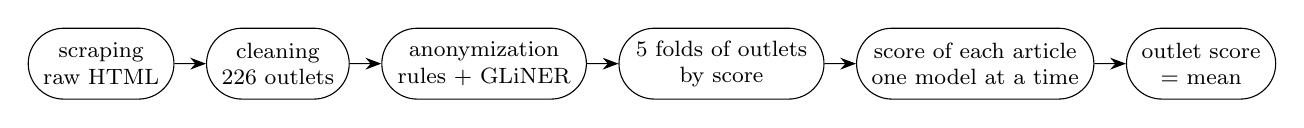
\begin{tikzpicture}[node distance=4mm, box/.style={draw, rounded rectangle, align=center, font=\footnotesize,
  minimum height=9mm, inner sep=3pt}, >={Stealth[length=2mm]}]
\node[box] (s) {scraping\\raw HTML};
\node[box, right=of s] (c) {cleaning\\226 outlets};
\node[box, right=of c] (a) {anonymization\\rules + GLiNER};
\node[box, right=of a] (f) {5 folds of outlets\\by score};
\node[box, right=of f] (m) {score of each article\\one model at a time};
\node[box, right=of m] (o) {outlet score\\= mean};
\foreach \x/\y in {s/c, c/a, a/f, f/m, m/o} \draw[->] (\x) -- (\y);
\end{tikzpicture}}
\caption{The pipeline. Each box is a step, from the collected pages (left) to the score of each outlet
(right).}\label{fig:pipeline}
\end{figure}

\subsection{Experimental setup}\label{sec:setup}
We use a 5-fold cross-validation over outlets (Figure~\ref{fig:pipeline}). The outlets are sorted by score and, in
blocks of five, assigned at random to different folds, so that every fold has the same score distribution
(Figure~\ref{fig:dataset}c). Each model is trained on four folds (about 180 outlets and 20,000 articles) and tested on
the fifth, so every outlet is scored once by a model that never saw it. The settings of the linear models (the ridge
penalty and, for Mistral-Small-24B, the layer) are chosen on three inner folds of the training outlets. In training every
article counts once, while in the evaluation every outlet counts once. The models read the body of each article, not the
title. We compare:
\begin{itemize}
  \item \textbf{TF-IDF + ridge:} word uni- and bi-grams with a ridge regression~\cite{hoerl1970ridge}, the standard
        strong baseline for vocabulary, topic and style.
  \item \textbf{Frozen language models + ridge:} a pretrained model, not trained on our data, turns each article into a
        vector, and a ridge regression on these vectors is the only part trained on the scores. We use the embedding
        models Qwen3-Embedding-8B and Qwen3-Embedding-0.6B~\cite{zhang2025qwen3}, given an instruction to represent the
        article for judging the reliability of its outlet; the base decoder Mistral-Small-24B~\cite{mistralsmall} in
        4-bit quantization~\cite{dettmers2023qlora}, through the mean hidden state of an intermediate
        layer~\cite{skean2025layer} (layer 27, chosen on the inner folds); and ModernBERT-base without training.
  \item \textbf{ModernBERT, fine-tuned:} the 150-million-parameter encoder~\cite{warner2024modernbert} trained end to end
        on the scores.
  \item \textbf{Mistral-Small-24B-Instruct, zero-shot:} the instruction-tuned Mistral is asked for the NewsGuard score of
        the site that published each article, with a prompt that describes the nine criteria (Supplementary
        Section~\ref{S-app:prompt}).
\end{itemize}
The two Qwen3 models differ in size, the two ModernBERT models only in their training, and the two Mistral models in how
they use the text. Supplementary Section~\ref{S-app:impl} gives all the settings. Every random choice is seeded, and the
predictions and the models of every fold are saved.

\subsection{Stage 1: article-level score estimation}\label{sec:stage1}
Table~\ref{tab:article} compares each test article with the score of its outlet. All models do better than chance, and
Mistral-Small-24B is the best (MAE 17.8, $\rho = 0.61$). A single article, however, is a weak signal: the trained models
put it within 20 points of the score of its outlet in 54--64\% of the cases, against 50\% without text. This is
expected, since every article inherits the score of its outlet, while a reliable outlet can publish a weak opinion piece
and an unreliable one a plain factual report. For this reason we judge each outlet on several articles.

\begin{table}[t]
\centering
\caption{Stage 1, single articles. Each row is a model; each of the 25,524 test articles is compared with the NewsGuard
score of its outlet. Lower MAE and higher $\rho$ and share within 20 points are better; the best value is in bold. The
rows above the line are baselines.}\label{tab:article}
\begin{tabular}{lccc}
\toprule
model & MAE (points) & Spearman $\rho$ & within 20 (\%) \\
\midrule
no text (training mean) & 23.0 & -- & 50.4 \\
Mistral-Small-24B-Instruct, zero-shot & 24.3 & 0.233 & 43.8 \\
\midrule
TF-IDF + ridge & 20.4 & 0.429 & 56.6 \\
ModernBERT (fine-tuned) & 20.4 & 0.458 & 58.0 \\
ModernBERT (frozen) + ridge & 20.9 & 0.403 & 55.0 \\
Qwen3-Embedding-0.6B (frozen) + ridge & 21.3 & 0.368 & 54.1 \\
Qwen3-Embedding-8B (frozen) + ridge & 19.4 & 0.525 & 59.3 \\
Mistral-Small-24B (frozen) + ridge & \textbf{17.8} & \textbf{0.614} & \textbf{63.5} \\
\bottomrule
\end{tabular}
\end{table}

\subsection{Stage 2: publisher-level score inference}\label{sec:stage2}
Table~\ref{tab:main} gives the main results, with the score of each outlet computed from all its articles, and
Figure~\ref{fig:scatter} shows the predictions. Averaging over the articles helps every model: from one article per
outlet to all of them, the error falls by 1.5--3.1 points, and $\rho$ rises from 0.62 to 0.735 for Mistral-Small-24B
and from 0.39 to 0.674 for TF-IDF.

\begin{table}[t]
\centering
\caption{Stage 2, outlets: the main results. Each row is a model; the score of an outlet is the mean of the predictions
for all its articles. Brackets give 95\% bootstrap intervals; $^\ast$ marks a model significantly better than TF-IDF
after Holm correction; the best value is in bold. The rows above the line are baselines.}\label{tab:main}
\resizebox{\linewidth}{!}{%
\begin{tabular}{lcccc}
\toprule
model & MAE (points) & Spearman $\rho$ & Kendall $\tau_b$ & within 20 (\%) \\
\midrule
no text (training mean) & 22.6 [20.7, 24.5] & $-$0.015 [$-$0.15, 0.11] & $-$0.012 [$-$0.11, 0.09] & 50.9 [44.2, 57.5] \\
no text (training median) & 22.1 [19.9, 24.4] & -- & -- & 54.0 [47.3, 60.6] \\
orientation only (training mean per orientation) & 18.5 [16.7, 20.5] & 0.362 [0.24, 0.48] & 0.260 [0.17, 0.35] & 64.2 [58.0, 70.4] \\
Mistral-Small-24B-Instruct, zero-shot & 24.4 [22.5, 26.2] & 0.348 [0.22, 0.46] & 0.246 [0.16, 0.33] & 41.6 [35.4, 48.2] \\
\midrule
TF-IDF + ridge & 17.8 [16.2, 19.6] & 0.674 [0.60, 0.73] & 0.480 [0.42, 0.54] & 61.5 [54.9, 67.7] \\
ModernBERT (fine-tuned) & 17.5 [15.8, 19.3] & 0.610 [0.52, 0.68] & 0.435 [0.37, 0.50] & 63.7 [57.5, 69.9] \\
ModernBERT (frozen) + ridge & 18.3 [16.6, 20.0] & 0.619 [0.53, 0.69] & 0.446 [0.38, 0.51] & 58.8 [52.7, 65.5] \\
Qwen3-Embedding-0.6B (frozen) + ridge & 18.8 [17.1, 20.6] & 0.626 [0.55, 0.69] & 0.439 [0.38, 0.50] & 57.1 [50.4, 63.7] \\
Qwen3-Embedding-8B (frozen) + ridge & 16.3$^\ast$ [14.8, 17.9] & 0.711 [0.65, 0.76] & 0.514 [0.46, 0.57] & \textbf{69.9}$^\ast$ [63.7, 75.7] \\
Mistral-Small-24B (frozen) + ridge & \textbf{15.8}$^\ast$ [14.3, 17.4] & \textbf{0.735} [0.67, 0.78] & \textbf{0.540} [0.48, 0.59] & 68.1 [61.9, 74.3] \\
\bottomrule
\end{tabular}}
\end{table}

\begin{figure}[t]
\centering
\includegraphics[width=\linewidth]{figures/scatter.pdf}
\caption{Predicted against true score. Each point is an outlet, placed at its NewsGuard score ($x$) and at the mean
prediction over its articles ($y$); the marker shape gives the NewsGuard level, and points on the dashed line are
predicted exactly.}\label{fig:scatter}
\end{figure}

\paragraph{Large frozen models are the best.} Mistral-Small-24B predicts the score of unseen outlets with an error of
15.8 points, against 17.8 for TF-IDF and 22.1 for the best constant, and ranks them with $\rho = 0.735$. Its error is
significantly lower than that of TF-IDF, by 2.0 points [$-2.9$, $-1.2$]; its higher $\rho$ ($+0.060$) and share within
20 points ($+6.6$) are not significant after the correction. Qwen3-Embedding-8B also lowers the error significantly
($-1.5$ [$-2.3$, $-0.7$]). The two large models do not differ significantly.

\paragraph{Small models are not better than TF-IDF.} Qwen3-Embedding-0.6B has an error 2.5 points higher than its
8-billion-parameter version and is no better than TF-IDF. ModernBERT is no better than TF-IDF either, frozen or
fine-tuned ($\rho$ 0.619 and 0.610, MAE 18.3 and 17.5). Fine-tuning fits the training articles well (an error of about 4
points), but this does not carry over to unseen outlets. The evidence separates small from large models; it does not show
a steady gain with size. Since we fine-tuned ModernBERT with fixed settings and one seed, this result concerns this small
encoder only.

\paragraph{Asking for the score does not work.} Asked directly for the score, the instruction-tuned Mistral ranks the
outlets with $\rho = 0.35$ and has a larger error than a constant (24.4 points), since 85\% of its answers are either 65
or 45. The same model family with a trained linear head is the best model of the study, in line with other tasks in
which a linear head on hidden states beats the text answers of language models~\cite{buckmann2025revealing}.

\paragraph{More than political orientation.} Predicting the mean score of the orientation of an outlet gives
$\rho = 0.36$. Every trained model ranks the outlets far better, and it also ranks them within each orientation
(Section~\ref{sec:orientation}).

\paragraph{Robustness.} All models compress their predictions towards the centre of the scale (Mistral-Small-24B
predicts between 37 and 96, Figure~\ref{fig:scatter}). A straight line fitted on the training folds re-maps the scores
and lowers every error by 1--3 points. After this recalibration Mistral-Small-24B remains better than TF-IDF ($-1.5$
[$-2.7$, $-0.4$]), while the advantage of Qwen3-Embedding-8B is no longer significant (Supplementary
Section~\ref{S-app:robust}). With four other random splits of the outlets, Mistral-Small-24B lowers the error of TF-IDF
by 2.0--2.3 points in each split (Supplementary Section~\ref{S-app:splits}).

\subsection{How many articles are needed}\label{sec:k}
To know how many articles must be collected for a new outlet, we predict each outlet from $k = 1, 2, 3, 5, 10, 20, 50$
of its articles, drawn at random 20 times, with the same draws for every model. Figure~\ref{fig:curves} shows the
results. Mistral-Small-24B is significantly better than TF-IDF for every $k$, on both the error and the ranking. With
one article per outlet its error is 17.3 points, against 20.5 for TF-IDF; with five articles it is 16.1, already
significantly lower than that of TF-IDF with all the articles (17.8). Qwen3-Embedding-8B is significantly better than
TF-IDF on the error for every $k$, and the small models are never better than TF-IDF. All curves flatten after about ten
articles, and the large models gain most when few articles are available, as for a new or small outlet.

\begin{figure}[t]
\centering
\includegraphics[width=\linewidth]{figures/curves.pdf}
\caption{Results by number of articles. The $x$ axis is the number of articles read per outlet; the $y$ axis is the
Spearman correlation (left) or the MAE (right) per outlet, averaged over 20 random draws. Each model has its own marker
and line; the dashed line is the no-text baseline.}\label{fig:curves}
\end{figure}

\subsection{Effect of the evaluation protocol}\label{sec:ladder}
Our protocol blocks three ways of recognizing an outlet: the same outlet in training, outlets of the same owner in
training, and names in the text. To measure each of them, we retrain the three ridge models under weaker protocols and
test them on the same articles and folds (Table~\ref{tab:ladder}):
\begin{itemize}
  \item \textbf{Article split:} the folds are drawn over articles, so every test outlet also has articles in training.
  \item \textbf{Sisters:} the training data also contain the 89 sister outlets removed by the cleaning, with all their
        articles, so 31 test outlets have a sister in training.
  \item \textbf{Original text:} no anonymization.
  \item \textbf{Rules only:} only the first two passes of the anonymization.
\end{itemize}

\begin{table}[t]
\centering
\caption{Effect of the evaluation protocol. Each row is a protocol, from the weakest (article split) to the protocol of
the paper (full protocol), always tested on the same articles and folds. Each cell gives the MAE or $\rho$ per outlet
and, in parentheses, the difference from the protocol that differs only in the protection removed (the original text
for the sisters, the full protocol for the others); $^\dagger$ marks a difference whose 95\% bootstrap interval excludes
zero. The lower blocks separate the outlets that have a sister from those that do not.}\label{tab:ladder}
\resizebox{\linewidth}{!}{%
\begin{tabular}{llcccccc}
\toprule
& & \multicolumn{2}{c}{TF-IDF} & \multicolumn{2}{c}{Qwen3-Embedding-8B} & \multicolumn{2}{c}{Mistral-Small-24B} \\
\cmidrule(lr){3-4}\cmidrule(lr){5-6}\cmidrule(lr){7-8}
outlets & protocol & MAE & $\rho$ & MAE & $\rho$ & MAE & $\rho$ \\
\midrule
all 226 & article split & 10.4 ($-$7.4)$^\dagger$ & 0.904 (+0.230)$^\dagger$ & 10.7 ($-$5.6)$^\dagger$ & 0.884 (+0.173)$^\dagger$ & 8.7 ($-$7.1)$^\dagger$ & 0.924 (+0.189)$^\dagger$ \\
 & sisters & 17.1 ($-$0.8) & 0.712 (+0.039)$^\dagger$ & 15.7 ($-$0.3) & 0.733 (+0.009) & 14.9 ($-$0.8) & 0.732 ($-$0.002) \\
 & original text & 18.0 (+0.1) & 0.673 ($-$0.001) & 16.0 ($-$0.3) & 0.724 (+0.013) & 15.7 ($-$0.1) & 0.734 ($-$0.001) \\
 & rules only & 17.7 ($-$0.1) & 0.679 (+0.005) & 15.9 ($-$0.4)$^\dagger$ & 0.724 (+0.013) & 15.7 ($-$0.1) & 0.734 ($-$0.001) \\
 & full protocol & 17.8 & 0.674 & 16.3 & 0.711 & 15.8 & 0.735 \\
\midrule
31 with a sister & sisters & 8.3 ($-$11.6)$^\dagger$ & 0.918 (+0.254)$^\dagger$ & 11.6 ($-$6.9)$^\dagger$ & 0.908 (+0.227)$^\dagger$ & 9.7 ($-$8.7)$^\dagger$ & 0.943 (+0.212)$^\dagger$ \\
 & original text & 19.9 & 0.664 & 18.4 & 0.681 & 18.3 & 0.732 \\
\midrule
195 without & sisters & 18.5 (+0.9)$^\dagger$ & 0.676 (+0.009) & 16.3 (+0.7)$^\dagger$ & 0.707 ($-$0.027) & 15.8 (+0.4) & 0.698 ($-$0.041)$^\dagger$ \\
 & original text & 17.7 & 0.667 & 15.6 & 0.734 & 15.3 & 0.739 \\
\bottomrule
\end{tabular}}
\end{table}

\paragraph{Same outlet.} Splitting articles instead of outlets lowers the error by 5.6--7.4 points and raises $\rho$ to
about 0.9, because the models recognize outlets they have already seen. Under this split TF-IDF, which can memorize the
vocabulary of each outlet, catches up with Qwen3-Embedding-8B (MAE 10.4 against 10.7).

\paragraph{Same owner.} Training on sister outlets has almost the same effect on the outlets that have one. For these 31
outlets the error falls by 7--12 points, to 8.3--11.6, close to the article split, while the other 195 outlets do not
improve. Half of the test articles of these 31 outlets have a near copy among the articles of their sisters, and sisters
usually share their rating: 23 of the 31 outlets have exactly the score of all their sisters. The gain is largest where
the articles of the sisters are most similar to the test articles, as Zhou et al.~\cite{zhou2021hidden} found for sites
with the same label (Supplementary Section~\ref{S-app:sisters}).

\paragraph{Names.} Masking the names, instead, changes the error by at most 0.4 points and no $\rho$ significantly.
Leaving out the 16 outlets whose brand name of two or more words is still in the text barely changes the advantage of
Mistral-Small-24B over TF-IDF (1.8 points instead of 2.0). The models therefore do not rely on the masked names, nor
mainly on what they may know about an outlet from pretraining: from the domain name alone, the frozen models rank the
outlets with $\rho = 0.35$--$0.39$, about as well as the orientation alone (Supplementary Section~\ref{S-app:robust}). An
earlier rule-based anonymization gives the same results (Supplementary Section~\ref{S-app:anon}).

\paragraph{Boilerplate.} Some outlets repeat the same lines in many articles, such as invitations to subscribe to a
newsletter, donation appeals and disclaimers, and the anonymization does not remove them. These lines (repeated in at
least three articles and in 5\% of the articles of an outlet) are 3.0\% of the words, and TF-IDF retrained without them
has about the same error (17.5 against 17.8). Mistral-Small-24B predicts with a linear function of the mean of its token
states, so we can measure exactly how much each token contributes to a prediction, as explanation methods
do~\cite{kozik2024explainability}. These lines move a prediction by 1.9 points on average, while the predictions have a
standard deviation of 17.5 points. The models use the boilerplate a little, but their predictions come mostly from the
body of the articles (Supplementary Section~\ref{S-app:reading}).

\subsection{Errors by reliability level}\label{sec:errors}
Figure~\ref{fig:errors}a shows the mean signed error per NewsGuard level. All models pull their predictions towards the
centre of the scale. The least reliable outlets are overestimated ($+31$ points for Mistral-Small-24B in the 0--39 band),
the outlets with a perfect score are underestimated ($-19$), and the middle of the scale (60--74) is predicted almost
without bias. For Mistral-Small-24B, one point of NewsGuard score moves the prediction by only 0.37 points on average.
The extremes are hard to predict for two reasons. They depend on criteria that single articles hardly show, such as the
repeated publication of false content or the disclosure of ownership, and the models are trained on single articles,
whose scores are then averaged: the compression is the same per article and per outlet. The ranking metrics are not affected, and the larger models compress less (Supplementary Section~\ref{S-app:errors}
gives the values for every model).

\begin{figure}[t]
\centering
\includegraphics[width=\linewidth]{figures/errors.pdf}
\caption{Errors by level and orientation, one bar per model. (a) Mean signed error (predicted minus true score) per
NewsGuard level: bars above zero are overestimates. (b) Mean signed error per political orientation after removing its
linear dependence on the true score, that is, at equal NewsGuard score. (c) Spearman correlation within the outlets of
each orientation, with 95\% bootstrap intervals.}\label{fig:errors}
\end{figure}

\subsection{Influence of political orientation}\label{sec:orientation}
Orientation and reliability are associated in our data, with a mean score of 80 for the left-leaning outlets and for
those without orientation and of 54 for the right-leaning ones. We therefore check whether the models treat the
orientations equally.

\paragraph{Ranking within an orientation.} All models rank the outlets within each orientation
(Figure~\ref{fig:errors}c), so they do more than recognize the political side. Mistral-Small-24B reaches $\rho = 0.62$
among the right-leaning outlets, 0.63 among those without orientation and 0.38 among the left-leaning ones, whose scores
are concentrated in the two highest levels.

\paragraph{Errors at equal score.} To compare outlets with the same NewsGuard score, we remove from the signed error its
linear dependence on the true score (Figure~\ref{fig:errors}b). Mistral-Small-24B then predicts the left-leaning outlets
5.2 points too high and the right-leaning ones 4.3 points too low, a gap of 9.6 points [6.7, 12.3], and 8.7--8.8 with
other ways of controlling for the score. The other trained models have gaps of 4.5--8.4 points, the zero-shot model none
(0.1). The compression alone does not create a gap. A plausible cause is that a model, when uncertain, moves an outlet
towards the outlets that write like it, which tend to share its orientation; a predictor that did this fully would have a gap of 12.6 points (Supplementary Section~\ref{S-app:errors}).

\paragraph{Calibration.} Comparing outlets with the same \emph{prediction} instead, the true scores of left- and
right-leaning outlets differ by only 0.8 points for Mistral-Small-24B [$-7.5$, 8.9]. We find no evidence that its
predictions mean different things for the two groups, while the difference is significant for the fine-tuned ModernBERT,
the small frozen models and the zero-shot model. When the groups have different mean scores, the two views cannot in
general be equal at the same time~\cite{kleinberg2017inherent,chouldechova2017fair}. In practice, a system built on these
models gives a right-leaning outlet about 9 points less than a left-leaning outlet with the same NewsGuard score, and
this must be considered when the predictions are used to choose which outlets to review.

% =====================================================================================================================
\section{Released Resources and Demonstration Tool}\label{sec:tool}
We release two repositories (Supplementary Section~\ref{S-app:tool} and Supplementary Table~\ref{S-tab:release}). The
first contains the pipeline and the code of every table and figure
(\url{https://github.com/bianchi-john/PublisherClassification}). The second contains the four main models of
Table~\ref{tab:main} in their five fold versions, the out-of-fold predictions for every article, the split of the
outlets (\url{https://github.com/bianchi-john/publisher-evaluation}\todo{publish the tool repository and check the link})
and \emph{Publisher Evaluation}, a tool that runs on the user's machine. The tool extracts, checks and anonymizes the
text of new articles as in the paper, shows what the models read, and scores it with the models chosen by the user,
never scoring one of the 226 outlets with a model that saw it in training. The NewsGuard ratings and the texts of the
articles are not released; the articles can be collected again from their URLs.

% =====================================================================================================================
\section{Discussion and Conclusion}\label{sec:conclusion}
We asked whether the NewsGuard score of a news outlet never seen in training can be predicted from its anonymized
articles. It can, in part. A large language model used as a frozen encoder, with a linear head trained on the scores,
predicts the score with an error of 15.8 points, against 17.8 for TF-IDF and 22.1 for a constant, and explains about
half of its variance ($R^2 = 0.48$). A few articles per outlet are enough, and more than about ten add little.

Three findings stand out. First, only large pretrained models do better than TF-IDF; small encoders, frozen or
fine-tuned, do not, and asking a model for the score does not work. A plausible explanation, which we cannot prove, is
that large models represent how claims are sourced and how arguments are built better than word counts and small
encoders do. Second, the evaluation protocol matters as much as the model. Training on the same outlet, or on outlets of
the same owner, lowers the error by 6--12 points, while masking the names changes it little, so outlet-disjoint splits,
deduplication across outlets and ownership groups are needed for realistic results. Third, the predictions are
compressed towards the centre of the scale and depend on orientation: at equal score, right-leaning outlets get about 9
points less than left-leaning ones.

Since the score is predicted within 20 points for about two outlets in three, and some criteria of the rating are
invisible in the text, these models should not replace the raters. Their natural use is to rank unrated outlets, so that
human raters can review the least reliable ones first, while keeping the gap between orientations under control.

\paragraph{Limitations.} The study uses one rater at one point in time and English-language political outlets only; the
open aggregate ratings of Lin et al.~\cite{lin2023high}, which include NewsGuard, could support a public replication.
With 226 outlets the intervals are wide, and most differences in ranking are not significant. The labels of the articles
are inherited from their outlets. The anonymization leaves the style, some brand names and the social-media handles, and
the ownership groups are those recorded by NewsGuard. The least reliable outlets are under-represented: re-weighted to
the outlets we could not collect, the expected error is about 20 points for Mistral-Small-24B and 23 for TF-IDF
(Supplementary Section~\ref{S-app:robust}). The protocol was developed on the same outlets (Supplementary
Section~\ref{S-app:tried}). Finally, the language models may know some outlets from their pretraining, although 96\% of
the articles were published after the release of every model we use and the domain name alone gives a much weaker
ranking than the text. Future work should extend the study to other languages, topics and raters, test the fine-tuning
of large models, and add signals that the text does not carry, such as ownership transparency or citation networks.

\paragraph{Ethics and data availability.}
The NewsGuard ratings were licensed to the authors for research. They cannot be redistributed, but the licence allows
the release of the models and of the predictions derived from them. The articles were collected from public pages,
without bypassing paywalls or logins, and their text is not redistributed. The study involves no human participants,
and the names of journalists are masked before the models read the articles. The predictions concern organizations, but
they could harm an outlet if used as ratings: they are meant to support human raters, should never be used to sanction
or label an outlet without human review, and should be monitored across political orientations. Like other text
classifiers, the models could also be fooled by an outlet that changes the few words that move a prediction, words that
explanation methods make easy to find~\cite{kozik2024explainability}. The code and the models are released under the
Apache-2.0 licence, and the predictions and the split under CC BY 4.0.

\section*{Acknowledgments}
This work is partially supported by IIT-CNR internal project SIMULARE `SIMULAzione delle Reazioni alla
disinformazionE con LLM'.

\bibliographystyle{plainnat}
\bibliography{references}

\end{document}
